\documentclass[11pt,a4paper]{report}

\usepackage[utf8]{inputenc}
\usepackage[T1]{fontenc}
\usepackage[english]{babel}
\usepackage[left=1in, right=1in, top=1in, bottom=1in]{geometry}
\usepackage{graphicx}
\usepackage{blindtext, amssymb, graphicx, mathtools, amsmath, listings, float, amsthm, tikz, multicol}
\usepackage{booktabs}
\usepackage{hyperref}
\usepackage{xcolor}
\usepackage{caption}
\usepackage{subcaption}
\usepackage{listings}
\usepackage{xcolor}



\newcommand{\N}{\mathcal{N}}
\newcommand{\Z}{\mathbb{Z}}
\newcommand{\R}{\mathbb{R}}
\newcommand{\G}{\mathbb{G}}
\renewcommand{\L}{\mathcal{L}}
\renewcommand{\l}{\ell}
\newcommand{\E}[1]{\mathbb{E}\left[ #1 \right]}
\newcommand{\var}[1]{\text{Var}\left( #1 \right)}
\newcommand{\cov}[2]{\text{Cov}\left( #1, #2 \right)}
\newcommand{\const}{\text{const}}


\newcommand{\pdf}[1]{f_{#1}}
\newcommand{\cdf}[1]{F_{#1}}

\newcommand{\disp}{\displaystyle}


\renewcommand{\P}{\mathbb{P}}
\renewcommand{\leq}{\leqslant}
\renewcommand{\geq}{\geqslant}


\newcommand{\Solution}{\[\textbf{ \ Solution:}\]}



\definecolor{codegreen}{rgb}{0,0.6,0}
\lstset{
    basicstyle=\ttfamily\small,
    keywordstyle=\color{blue},
    commentstyle=\color{codegreen},
    breaklines=true,
    frame=single
}


\usepackage{titlesec}

% Настройка команды \chapter
\titleformat{\chapter}[display]
  {\normalfont\huge\bfseries}{\chaptertitlename\ \thechapter}{20pt}{\Huge}
  
% Управление отступами: {левый}{перед}{после}
\titlespacing*{\chapter}{0pt}{-20pt}{30pt}



\title{Numerical Simulation of Pollutant Dispersion in a T-shaped Cavity using CFD Methods}
\author{}
\date{\today}





\begin{document}

\maketitle

\begin{abstract}
This report presents the numerical investigation of pollutant dispersion within a T-shaped building geometry, inspired by the benchmarks of Kikumoto and Ooka. The study utilizes Computational Fluid Dynamics (CFD) to analyze the transport of sulfur hexafluoride ($SF_6$) under transient wind conditions. ...
\end{abstract}
\tableofcontents
\newpage



\chapter{Introduction}

\section{Background and Motivation}
In modern urban environments, populations spend a significant portion of their time within complex architectural structures. Consequently, understanding the mechanisms of pollutant transport and gas leak propagation is critical for public safety and urban planning. In environments with complex geometries, such as T-shaped intersections or street canyons, aerodynamic "trapping" effects can occur. These stagnant zones lead to the accumulation of hazardous substances, creating localized high-concentration areas. This study evaluates the dispersion characteristics within a T-shaped building configuration to identify potential stagnation points and plume evolution behavior.


\section{Problem Statement}
The core of this research is based on the experimental and numerical benchmarks established by Hideki Kikumoto and Ryozo Ooka. We focus on a T-shaped building model where a primary airflow interacts with a secondary source of pollutant gas. In real-world scenarios, such configurations represent street canyons, industrial hallways, or complex ventilation ducts where stagnant zones can lead to dangerous concentrations of toxic gases.

\section{Sulfur hexafluoride ($SF_6$) as a Pollutant}
In our simulation, we chose Sulfur hexafluoride as the gas that leaks into the urban area. Sulfur hexafluoride ($SF_6$) is a colorless, odorless, non-toxic, and extremely stable synthetic gas. It is also known as the world's most potent greenhouse gas, with a global warming potential 23 500 times greater than ($CO_2$)
and an atmospheric lifetime exceeding 1 000 years. Our goal was to see how this gas moves through the building when a steady wind blows. By watching how its concentration changes, we can identify which parts of the area become dangerous first.

\section{Objectives}
The main objectives of this study are:
\begin{itemize}
    \item To design urban area's 3D geometry.
    \item To implement Computational Fluid Dynamics (CFD) setup in ANSYS Fluent capable of handling transient species transport.
    \item To optimize numerical parameters to ensure high precision convergence.
    \item To visualize the evolution of the pollutant plume and identify areas of high accumulation.
\end{itemize}

\chapter{Geometry and Mesh}

\section{Geometry and Computational Domain}

The numerical investigation is based on an idealized Urban Street Canyon (USC) configuration. The geometry is defined by a unity aspect ratio, where the street width ($W$) and building height ($H$) are both set to 18~m ($W/H = 1$). This specific configuration was chosen to maintain consistency with the experimental wind-tunnel (WT) data provided by the University of Karlsruhe, Germany. 

The validation of the current numerical model relies on the comparison between computational results and concentration measurements available in the public scientific database, as discussed in previous studies comparing \textit{Reynolds-Averaged Navier-Stokes} (RANS) and \textit{Large Eddy Simulation} (LES) approaches for atmospheric pollutant dispersion.

The first phase of the project involved the construction of a 3D model representing the street canyon area. The flow domain and its respective boundary conditions are defined as follows:

\begin{itemize}
    \item \textbf{Main Air Inlet:} A velocity-inlet profile representing the atmospheric boundary layer.
    \item \textbf{Outlet:} A zero-static pressure outlet to allow for fully developed flow.
    \item \textbf{Pollutant Sources:} Two parallel line sources located at the ground level between the buildings to simulate vehicular emissions ($SF_6$). Each source has a width of $0.12H$ and extends beyond the building length by 10\% to minimize boundary interference.
\end{itemize}

The detailed dimensions of the computational domain and the nested subdomains are illustrated in Figure 2.1.

\begin{figure}[htbp]
    \centering
    \begin{subfigure}[b]{0.48\textwidth}
        \centering
        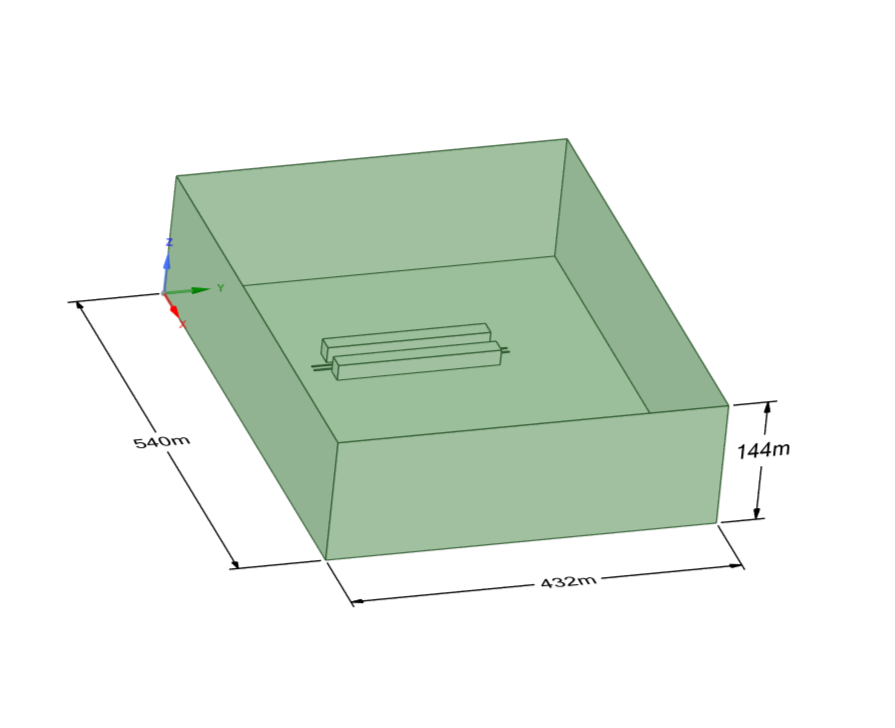
\includegraphics[width=\textwidth]{domain_setup.png}
        \caption{Top view of the domain}
        \label{fig:domain:top}
    \end{subfigure}
    \hfill
    \begin{subfigure}[b]{0.48\textwidth}
        \centering
        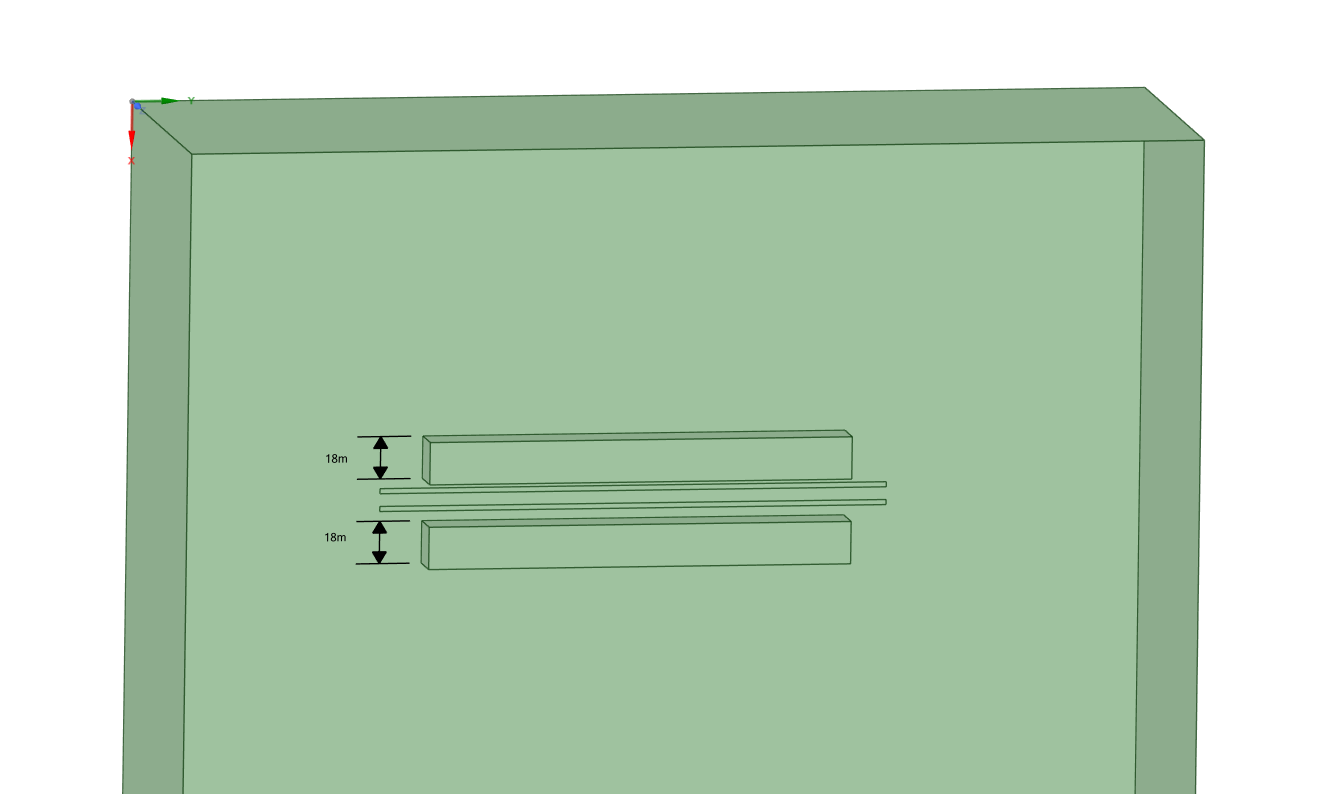
\includegraphics[width=\textwidth]{subdomain_setup.png}
        \caption{subdomain }
        \label{fig:domain:side}
    \end{subfigure}

    \caption{Computational domain setup: (a) layout and subdomains; (b) applied boundary conditions and line source locations.}
    \label{fig:domain_full}
\end{figure}


\newpage
\section{Computational Mesh}
To achieve a balance between computational cost and spatial resolution, a hybrid hexa-dominant mesh was generated. The domain was discretized using a multi-zone approach, where the region surrounding the T-shaped building and the pollutant sources (the street canyon) was heavily refined to capture the complex flow physics and high concentration gradients.

The mesh parameters are summarized as follows:
\begin{itemize}
    \item \textbf{Global Mesh Size:} $H/4.5 \approx 4$~m, ensuring a baseline resolution for the far-field flow.
    \item \textbf{Refinement Zone (Sub-mesh):} Within the street canyon and near building surfaces, the element size was reduced to $H/9 \approx 2$~m.
    \item \textbf{Boundary Layer Treatment:} To accurately resolve the viscous sublayer and pressure-driven separation at the building corners, 5 inflation layers were applied to all solid wall boundaries.
    \item \textbf{Mesh Statistics:} The final discretized domain consists of approximately 591,495 nodes and 3,388,605 elements.
\end{itemize}

\bigskip

\section{Mesh Quality Assessment}
The accuracy and stability of the numerical solution are directly influenced by the quality of the computational mesh. In this study, three primary metrics were utilized to evaluate the mesh: Element Quality, Aspect Ratio, and Skewness.

\begin{itemize}
    \item \textbf{Element Quality:} This composite metric evaluates the shape of the element on a scale from 0 to 1, where 1 represents a perfect equilateral cell and 0 indicates a degenerate cell with zero or negative volume. For 3D elements, it is calculated based on the ratio of the volume to the square root of the cube of the sum of the square of the edge lengths. 
    \item \textbf{Aspect Ratio:} Defined as the ratio of the longest edge length to the shortest edge length of an element. High aspect ratios can lead to numerical instability, particularly in regions with high flow gradients; however, values observed within the boundary layer (inflation layers) are within standard limits for the PISO solver.
    \item \textbf{Skewness:} This metric measures how close an element is to its ideal equilateral form. A skewness of 0 represents an ideal cell, while values approaching 1 indicate highly distorted elements that may hinder convergence.
\end{itemize}

The statistical distribution of these metrics is illustrated in Figure 2.2. The mean values recorded—0.77 for Element Quality, 1.83 for Aspect Ratio, and 0.22 for Skewness—demonstrate a high-quality discretization suitable for transient species transport analysis.

\newpage


\begin{figure}[htbp]
    \centering
    \begin{subfigure}[b]{0.32\textwidth}
        \centering
        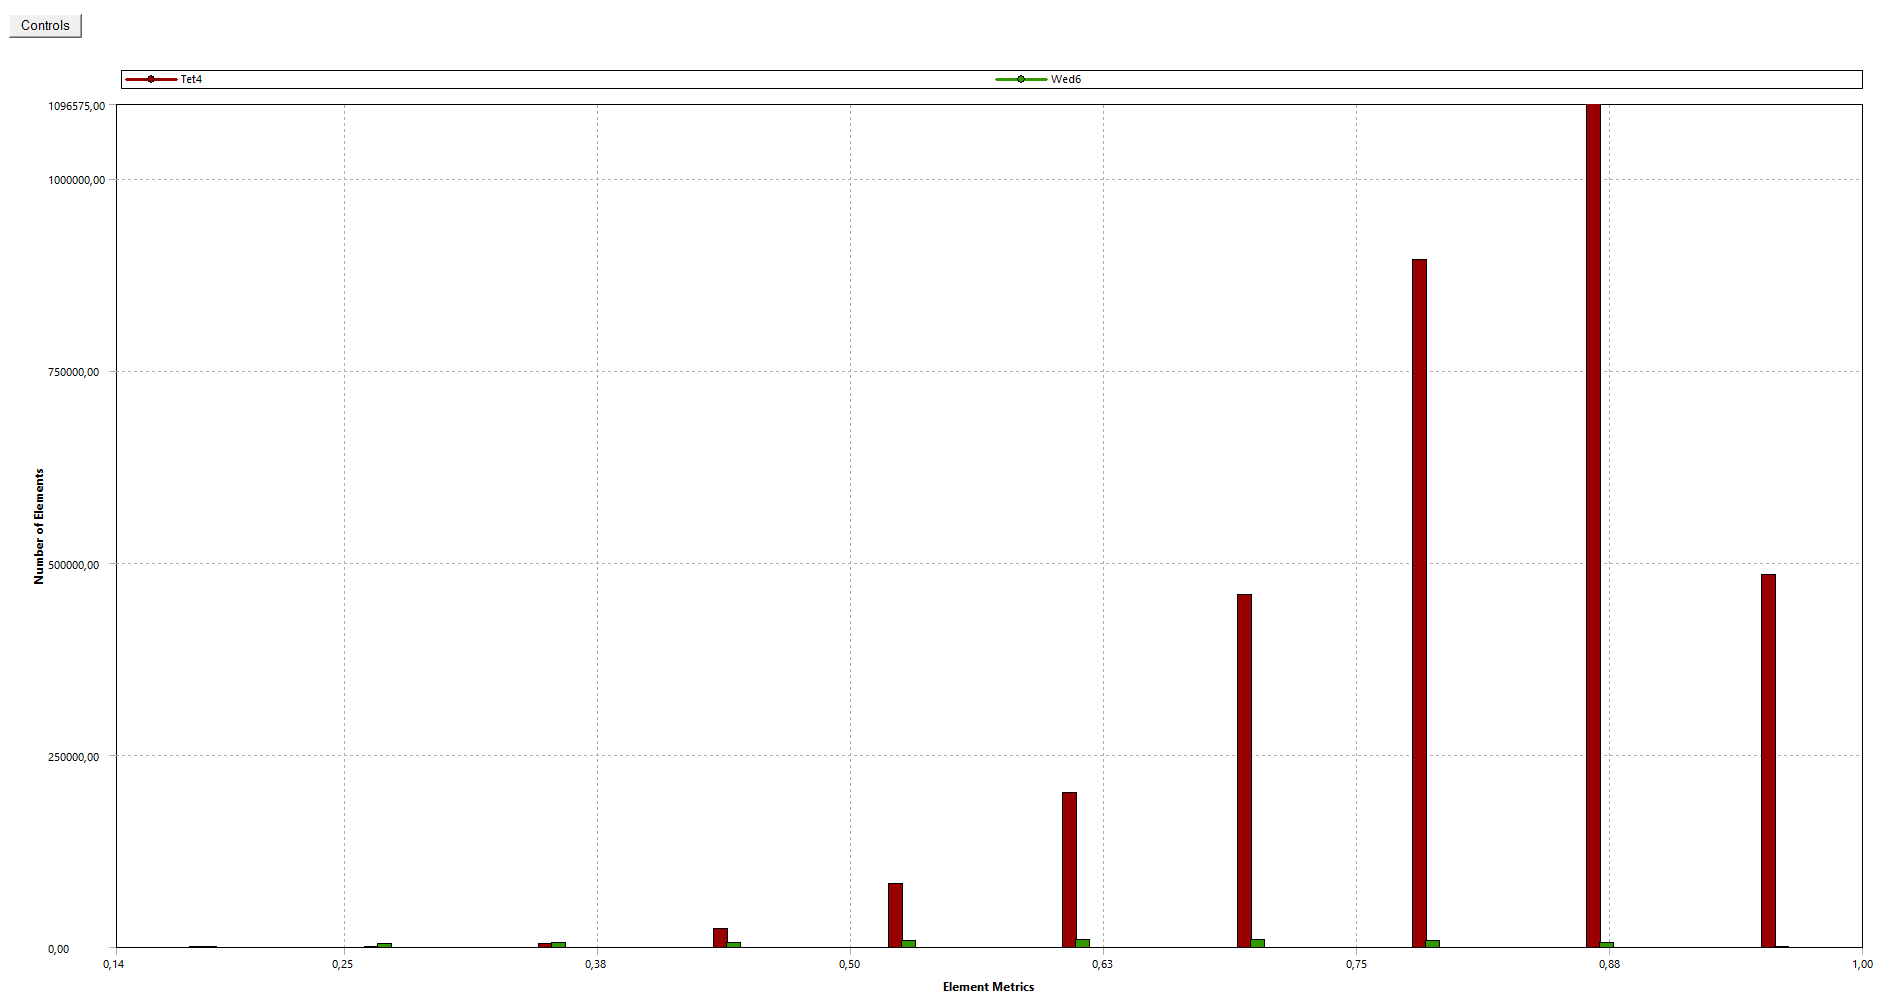
\includegraphics[width=\textwidth]{elem-quality.png}
        \caption{Element Quality}
        \label{fig:quality:element}
    \end{subfigure}
    \hfill
    \begin{subfigure}[b]{0.32\textwidth}
        \centering
        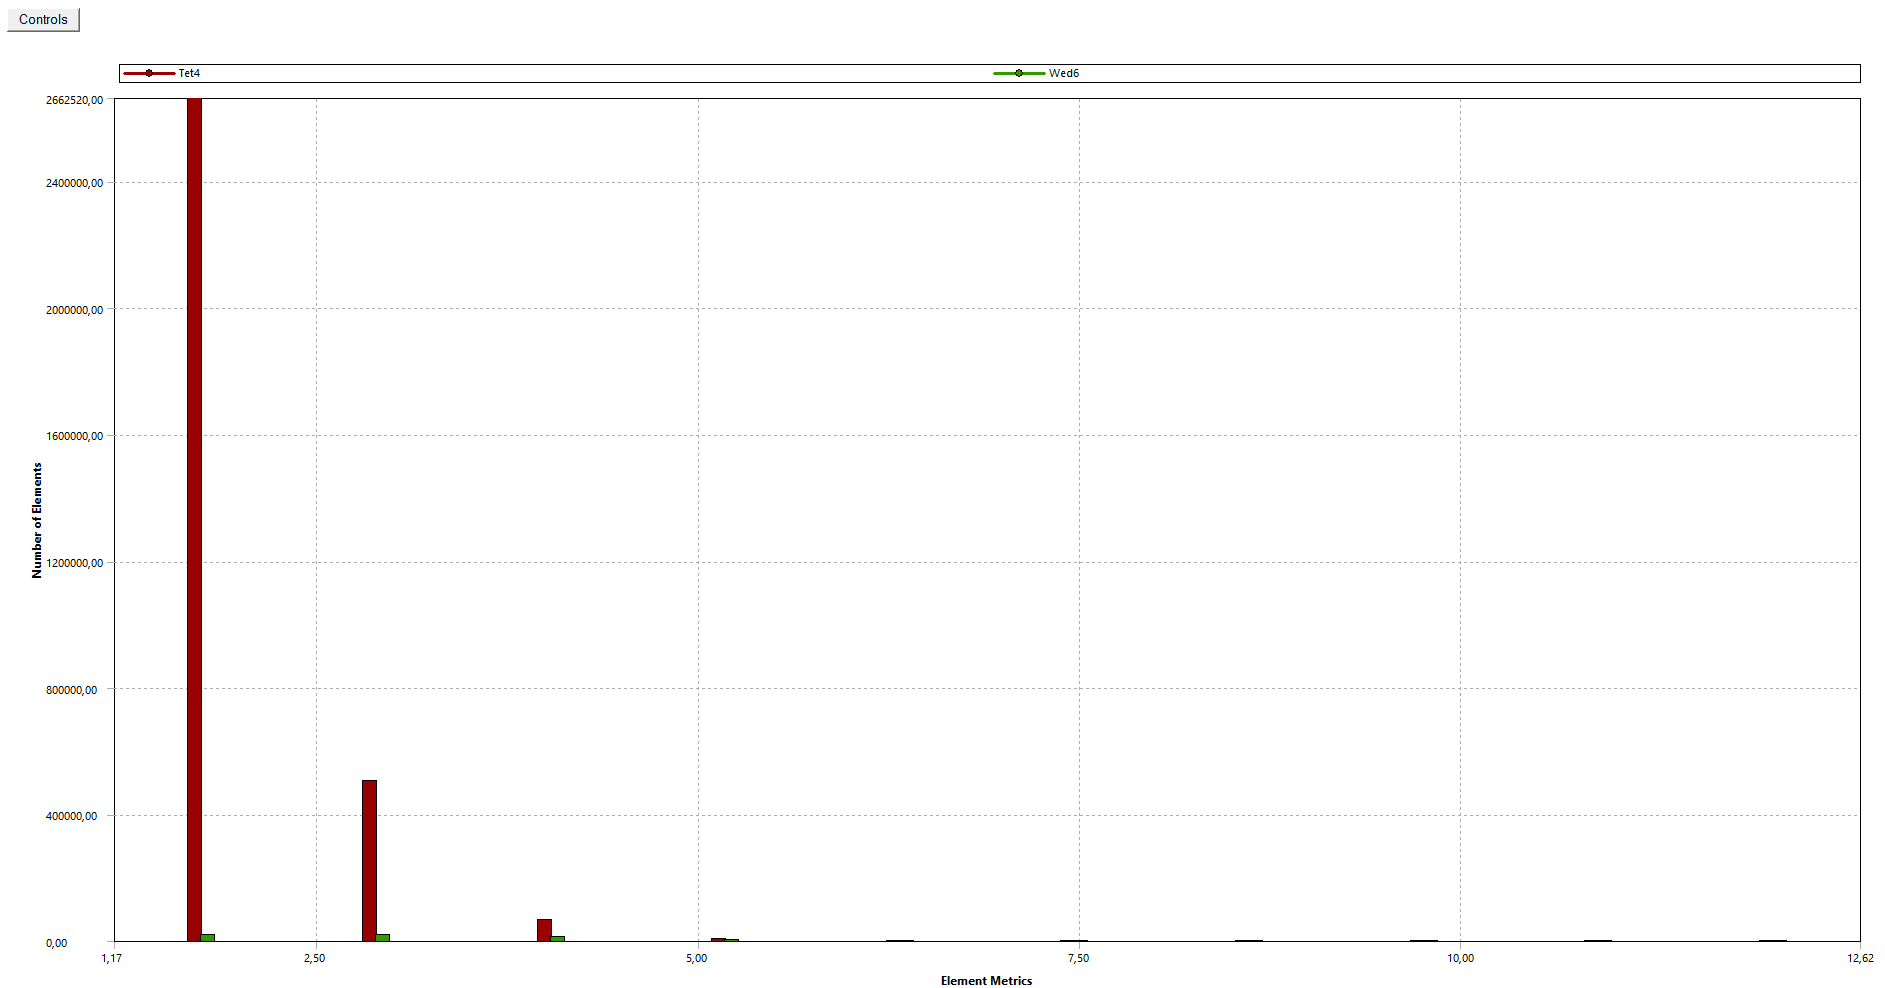
\includegraphics[width=\textwidth]{aspect-ratio.png}
        \caption{Aspect Ratio}
        \label{fig:quality:aspect}
    \end{subfigure}
    \hfill
    \begin{subfigure}[b]{0.32\textwidth}
        \centering
        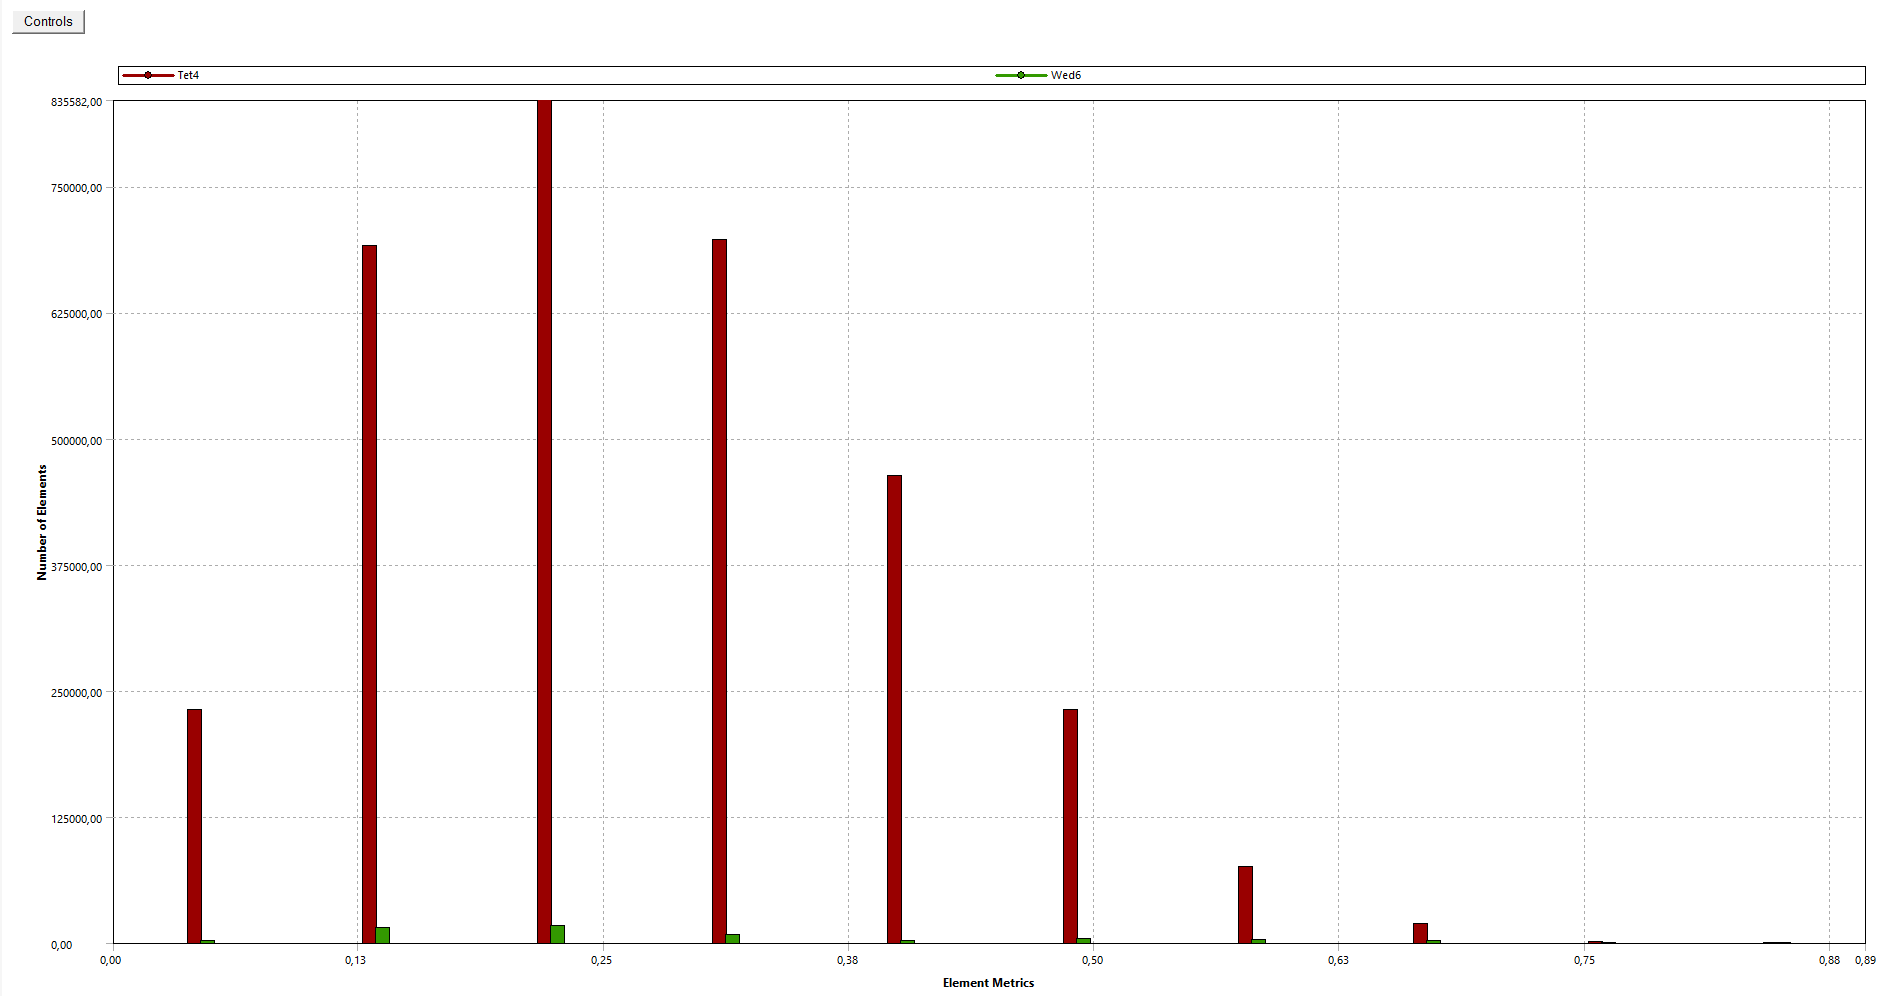
\includegraphics[width=\textwidth]{skewness.png}
        \caption{Skewness}
        \label{fig:quality:skew}
    \end{subfigure}
    \caption{Mesh quality histograms: (a) Element Quality distribution (Mean: 0.77); (b) Aspect Ratio distribution (Mean: 1.83); (c) Skewness distribution (Mean: 0.22).}
    \label{fig:mesh_metrics_histograms}
\end{figure}

The minimum orthogonal quality of $0.106$ and the maximum aspect ratio of $31.65$ (localized at the walls) ensure that the mesh is robust enough to handle the complex turbulent structures within the T-shaped geometry.

The majority of elements maintain a skewness value below 0.25 and an aspect ratio near unity in the critical regions, which minimizes numerical diffusion during the transient species transport simulation.

\chapter{Numerical Setup and Boundary Conditions}

\section{Governing Equations}
The fluid flow is governed by the steady-state 3D Reynolds-Averaged Navier-Stokes (RANS) equations. Since the simulation is performed under steady conditions, the time-dependent terms are neglected. The mass conservation and momentum equations are expressed as follows:

\begin{equation}
    \nabla \cdot (\rho \mathbf{u}) = 0
\end{equation}

\begin{equation}
    \nabla \cdot (\rho \mathbf{u} \mathbf{u}) = -\nabla p + \nabla \cdot (\tau) + \rho \mathbf{g}
\end{equation}


For the pollutant dispersion, a species transport model without chemical reactions was employed. The local mass fraction of the pollutant ($SF_6$), denoted as $Y_i$, is predicted through the solution of a convection-diffusion equation:

\begin{equation}
    \frac{\partial}{\partial t}(\rho Y_i) + \nabla \cdot (\rho \mathbf{u} Y_i) = -\nabla \cdot \mathbf{J}_i + S_i
\end{equation}
where $\mathbf{J}_i$ is the diffusion flux of the species.





\section{Inlet Boundary Conditions and UDF}
To simulate a realistic Atmospheric Boundary Layer (ABL), the inlet velocity, turbulent kinetic energy ($k$), and dissipation rate ($\varepsilon$) were prescribed using a User-Defined Function (UDF). The velocity profile follows a power law representing neutral atmospheric stability.

The profiles are defined as:
\begin{itemize}
    \item \textbf{Inlet Velocity:} $u(z) = 4.7 \bigl( \frac{z}{18} \bigr)^{0.3}$, where 18 m is the reference height ($H$).
    \item \textbf{Turbulent Kinetic Energy (k):} Derived from the friction velocity $u_* = 0.54$ m/s, accounting for the boundary layer depth $\delta = 144$ m.
    \item \textbf{Dissipation Rate ($\varepsilon$):} Calculated to ensure an equilibrium ABL, preventing the decay of turbulence as the flow traverses the domain.
\end{itemize}

\bigskip
The inlet wind speed was assumed to follow a power law profile:

\begin{equation}
  u(z) = 4.7 \Bigl( \frac{z}{18} \Bigr)^{0.3} \text{ms}^{-1} 
  \label{eq: Inlet wind speed}
\end{equation}

\bigskip

Turbulent kinetic energy and dissipation rate profiles were specified as follows:

\begin{equation}
  k = \frac{u^2_*}{\sqrt{C_\mu}} \Bigl( 1 - \frac{z}{\delta} \Bigr)
  \label{eq:Turbulent kinetic energy}
\end{equation}

\begin{equation}
  \varepsilon = \frac{u_*^3}{\kappa z}  \Bigl( 1 - \frac{z}{\delta} \Bigr)
  \label{eq: Dissipation rate}
\end{equation}

\bigskip

Where $\delta$ is the boundary layer depth ($= 144$ m), $u_* = 0.54$ m s$^{-1}$ is
the friction velocity and  
$\kappa$ is the von Karman constant (0.4), \ $C_\mu = 0.09$.

\bigskip

\begin{lstlisting}[language=C, caption={UDF}]
#include "udf.h"

#define U_STAR 0.54
#define DELTA 144.0
#define KAPPA 0.4
#define CMU 0.09

DEFINE_PROFILE(velocity_inlet, thread, position)
{
  real x[ND_ND], z;
  face_t f;
  begin_f_loop(f, thread)
  {
    F_CENTROID(x, f, thread);
    z = x[2]; 
    if (z < 0.01) z = 0.01;
    F_PROFILE(f, thread, position) = 4.7 * pow(z / 18.0, 0.3);
  }
  end_f_loop(f, thread)
}

DEFINE_PROFILE(k_profile, thread, position)
{
  real x[ND_ND], z;
  face_t f;
  begin_f_loop(f, thread)
  {
    F_CENTROID(x, f, thread);
    z = x[2];
    if (z > DELTA) z = DELTA;
    F_PROFILE(f, thread, position) = (pow(U_STAR, 2) / sqrt(CMU)) * (1.0 - z/DELTA);
  }
  end_f_loop(f, thread)
}

DEFINE_PROFILE(eps_profile, thread, position)
{
  real x[ND_ND], z;
  face_t f;
  begin_f_loop(f, thread)
  {
    F_CENTROID(x, f, thread);
    z = x[2];
    if (z < 0.1) z = 0.1; 
    if (z > DELTA) z = DELTA * 0.99;

    F_PROFILE(f, thread, position) = (pow(U_STAR, 3) / (KAPPA * z)) * (1.0 - z/DELTA);
  }
  end_f_loop(f, thread)
}
\end{lstlisting}

\section{Boundary Conditions}
The boundary conditions were defined to accurately replicate the atmospheric boundary layer and the specific pollutant emission source:

\begin{itemize}
    \item \textbf{Main Inlet:} A velocity-inlet profile implemented via UDF with $u_* = 0.54$ m/s and a boundary layer depth $\delta = 144$ m (scaled to full-size geometry)[cite: 181].
    \item \textbf{Pollution Source:} A \textit{mass-flow-inlet} was used for the $SF_6$ release with a rate of $0.00015$ kg/s. The turbulence parameters at the source were set to a $2\%$ intensity and a turbulent viscosity ratio of $2.5$.
    \item \textbf{Outlet:} A \textit{pressure-outlet} was applied with a \textit{Radial Equilibrium Pressure Distribution} to account for the vertical pressure gradient. Backflow turbulence was set to $5\%$ intensity and a viscosity ratio of $10$.
    \item \textbf{Walls:} No-slip conditions were applied to all building and ground surfaces[cite: 168, 206].
\end{itemize}

\section{Solver Stability and Convergence}
To ensure stable convergence and prevent numerical oscillations during the steady-state iterations, the Under-Relaxation Factors (URF) were optimized. Higher values were assigned to the species and energy equations to prioritize their convergence after the flow field became partially developed.


\begin{table}[htbp]
    \centering
    \caption{Applied Under-Relaxation Factors}
    \label{tab:urf}
    \begin{tabular}{l|c}
        \hline
        \textbf{Variable} & \textbf{Factor Value} \\ \hline
        Pressure & $0.3$ \\
        Momentum & $0.7$ \\
        Turbulent Kinetic Energy ($k$) & $0.8$ \\
        Dissipation Rate ($\varepsilon$) & $0.8$ \\
        Air (Mass Fraction) & $0.9$ \\
        $SF_6$ (Mass Fraction) & $0.9$ \\
        Energy & $1.0$ \\ \hline
    \end{tabular}
\end{table}

The solution was considered converged when the scaled residuals for all equations reached a threshold of $1 \times 10^{-5}$. In addition to residuals, the mass fraction of $SF_6$ at the outlet was monitored to ensure it reached a steady-state value.

\section{Material Properties and Species Transport}
The dispersion study involves a mixture of air and Sulfur hexafluoride ($SF_6$) as a tracer gas. To accurately simulate the buoyancy effects, the following properties were implemented:
\begin{itemize}
    \item \textbf{Tracer Gas ($SF_6$):} The molecular weight is set to $146.06$ kg/kmol, making it approximately five times heavier than air[cite: 158]. The density is modeled using the ideal-gas law, and the viscosity is defined as $1.53 \times 10^{-5}$ Pa$\cdot$s.
    \item \textbf{Mixture Properties:} The background air viscosity is $1.7894 \times 10^{-5}$ kg/m$\cdot$s. The mass diffusivity for the $SF_6$-air mixture is specified as $9.5 \times 10^{-6}$ m$^2$/s[cite: 319].
    \item \textbf{Turbulent Schmidt Number:} Following the standard recommendations for atmospheric dispersion, the Turbulent Schmidt Number ($Sc_t$) is set to $0.7$[cite: 320].
\end{itemize}

\section{Solver Configuration}
The numerical solution was obtained using the following settings in ANSYS Fluent:
\begin{itemize}
    \item \textbf{Solver Type:} A pressure-based steady-state solver was employed[cite: 164, 274].
    \item \textbf{Gravity:} Gravity was enabled in the negative Z-direction ($-9.81$ m/s$^2$) to account for the settling of the heavy tracer gas.
    \item \textbf{Turbulence Model:} The standard $k-\epsilon$ model was used with the following constants: $C_\mu = 0.09$, $C_{1\epsilon} = 1.44$, and $C_{2\epsilon} = 1.92$[cite: 91].
    \item \textbf{Discretization:} Second-Order Upwind schemes were applied for momentum and species transport to ensure higher accuracy and stability[cite: 275].
\end{itemize}


% Boundary conditions:
% inlet: U_STAR = 0.54 m s^-1, DELTA = 0.5 m KAPPA (von Karman constant) = 0.4, Cmu = 0.09
% pollution inlet: mass-flow-inlet: 0.00015 kg/s, turbulent intensity: 2%, turbulent viscosity ratio: 2.5
% outlet: turbulent intensity: 5%, turbulent viscosity ratio: 10, Radial Equilibrium Pressure Dsitribution



% Under relaxation factors:
% Pressure 0.3
% Momentum 0.7
% Turbulent kinetic energy 0.8
% Dissipation rate 0.8
% air 0.9
% sf6 0.9
% energy 1




% Equations:
% Flow
% Turbulence
% air
% sf6
% energy


\end{document}